\documentclass[a4paper, czech]{article}

\title{Úloha č.10: Integrovaný koncový zesilovač 20\,W KMJ2005SX}
\author{Karolína Andrea Šebestová \and Jan Božejovský}
\date{Datum měření: 3.12.2024}

\usepackage[czech]{babel}
\usepackage{indentfirst}
\usepackage{graphicx}
\usepackage{float}
\usepackage[margin=1.5cm]{geometry}
\usepackage{booktabs}
\usepackage{amsmath}
\usepackage[dvipsnames, table]{xcolor}
\usepackage{multirow}
\usepackage{tabularray}
\usepackage{bold-extra}
\usepackage{circuitikz}
\usepackage{caption}
\usepackage{subcaption}
\usepackage[utf8]{inputenc}
\usepackage{array}
\usepackage{nicematrix}
\usepackage{gensymb}

\begin{document}

\maketitle

\section{Teoretický úvod}

\begin{figure}[H]
    \centering
    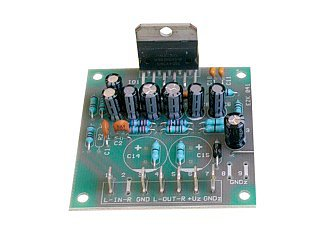
\includegraphics[]{kmj2005.jpg}
    \caption{Fotografie zhotoveného modulu KMJ2005SX}
\end{figure}

Zapojení tohoto modulu zesilovače vychází z doporučeného zapojení integrovaného
obvodu TDA2005 od společnosti STMicroelectronics.
U TDA2005 jsou dva koncové zesilovače.
Oba kanály jsou zapojeny zcela stejně.
Zesílení koncových stupňů je dáno rezistory R$_6$ až R$_9$.

\begin{figure}[H]
    \centering
    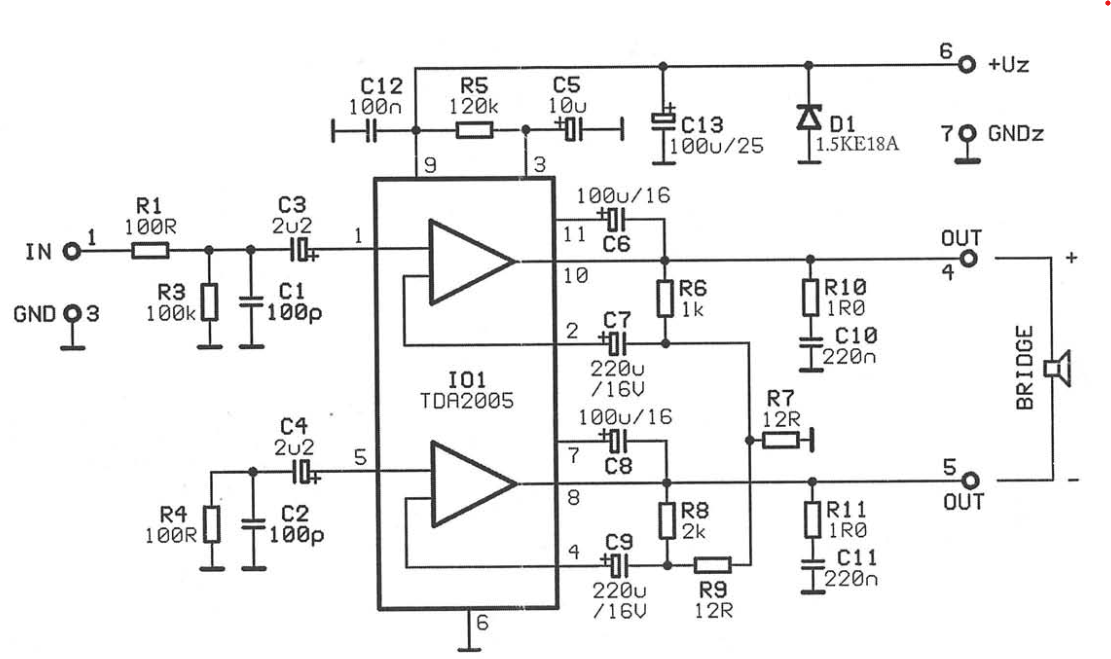
\includegraphics[width=0.6\textwidth]{schema.png}
    \caption{Schéma zapojení modulu KMJ2005SX}
\end{figure}

\section{Úkoly měření}

\begin{enumerate}
    \item Pro měření výstupního napětí zesilovače používejte vždy diferenční sondu. Tato sonda 10x zeslabuje a její BNC výstup musí být vždy zatížen 50\,$\Omega$ odporem. Na osciloskopu na kanálu, kde je sonda připojena, nastavte proto příslušný dělicí poměr sondy (10:1) a BNC výstup sondy zatižte 50\,$\Omega$ odporem v provedení BNC přes T rozbočku. Požádejte pro jistotu vyučujícího o instrukce k měření sondou, aby nedošlo k chybám. Jako zátěž simulující reproduktor mějte vždy k zesilovači připojený keramický výkonový rezistor 8\,$\Omega$. Experimentálně zjistěte velikosti vstupního sinusového napětí o frekvenci 1 kHz, kdy je na výstupu zesilovače výkon 4 W a 8 W do zátěže 8\,$\Omega$. Postupujte tak, že budete na generátoru postupně zvyšovat amplitudu sinusového signálu, až na výstupu zesilovače dosáhnete napětí odpovídající uvedeným výkonům. Platí vztah $P = U^2$/2 (pozor, U je zde efektivní hodnota, tedy RMS). Nezapomeňte aktivovat výstup generátoru pomocí stisku tlačítka Channel a volby Output On tlačítkem pod displejem. Výpočet výstupního napětí odpovídajícího výkonům 4 W a 8 W do zátěže 8\,$\Omega$ a zjištěná vstupní napětí uveďte v protokolu.
    \item Pomocí analyzátoru Bode 100 změřte frekvenční charakteristiky modulu a fáze přenosu (20 Hz - 100 kHz). Výstupní úroveň analyzátoru nastavte na -27 dBm.
    \item Pomocí analyzátoru Bode 100 změřte frekvenční charakteristiky modulu a fáze vstupní impedance (20 Hz - 100 kHz). Výstupní úroveň analyzátoru nastavte na -27 dBm.
    \item Zjistěte účinnost zesilovače pro výstupní výkon 4 W a 8 W jako poměr tohoto výstupního výkonu a příkonu dodávaného napájecím zdrojem. Tento příkon vypočítejte pomocí údajů na displeji zdroje.
    \item Změřte harmonické zkreslení (THD) na výstupu pro výstupní výkon 4 W a 8 W pomocí měřiče Tesla BM543. Do vstupu zesilovače přiveďte z generátoru sinusový průběh o kmitočtu 1 kHz a amplitudě odpovídající příslušnému výstupnímu výkonu. Výstup zesilovače přiveďte do vstupu měřiče Tesla BM543 opět pomocí diferenční sondy s T-článkem a 50\,$\Omega$ odporem. Před měřením zkreslení je nutno nastavit přepínač funkcí na LEVEL a přepínač rozsahů na 100 \% zkreslení (0,3 V). Ovládacími prvky SENSITIVITY (hrubě a jemně) nastavíme plnou výchylku měřidla, tedy na hodnotu jedna. Tlačítko způsobu ladění přepneme do polohy RUČNĚ (symbol ruky). Tím je přístroj převeden na ruční způsob měření zkreslení. Přepínač FREQUENCY nastavíme na „x 100 Hz“ a stříbrný kotouč s kmitočtovou stupnicí na 10. Tím naladíme filtr typu pásmová zádrž v měřiči na 1 kHz, abychom mohli odfiltrovat základní harmonickou složku signálu a změřit podíl vyšších harmonických, tedy THD. Přepínač funkcí nyní přepneme na DISTORTION METER. Jemným otáčením kotouče s kmitočtovou stupnicí okolo hodnoty 10 a najdeme minimum výchylky ručky. Postupně přepínáme rozsah měřiče ze 100 \% na jemnější a opět dostavováním stříbrného kotouče najdeme minimum výchylky ručky. Dále snižujeme výchylku ručky knoflíkem BALANCING (vnitřní červený je hrubě, vnější šedý je jemně) za dalšího průběžného zjemňování rozsahu měřiče. Je-li hodnota na měřiči menší než 5 \%, stlačením tlačítka AUT. zapneme automatické vyhledání zkreslení. Přepínač rozsahů případně dále přepneme k nižším hodnotám, až se ručička zastaví na odečitatelné hodnotě uvnitř stupnice měřidla. Zkreslení čteme na stupnici měřidla. Rozsah je určen postavením přepínače rozsahů v procentech. Požádejte pro jistotu vyučujícího o pomoc s tímto úkolem, aby nedošlo k chybám.
\end{enumerate}

\section{Seznam použitých přístrojů}

\begin{itemize}
    \item Laboratorní zdroj DF1731SB
    \item Signálový generátor Agilent 33521A
    \item Obvodový analyzátor Bode 100
    \item Diferenční sonda Agilent N2792A
    \item Digitální osciloskop Agilent DSO-X 2012A
    \item Poloautomatický zkresloměr Tesla BM 543
\end{itemize}

\section{Zpracování úkolů}

\subsection{Měření vstupního sinusového napětí (Úkol 1)}



\subsection{Měření frekvenční charakteristiky modulu a fáze přenosu (Úkol 2)}

\begin{figure}[H]
    \centering
    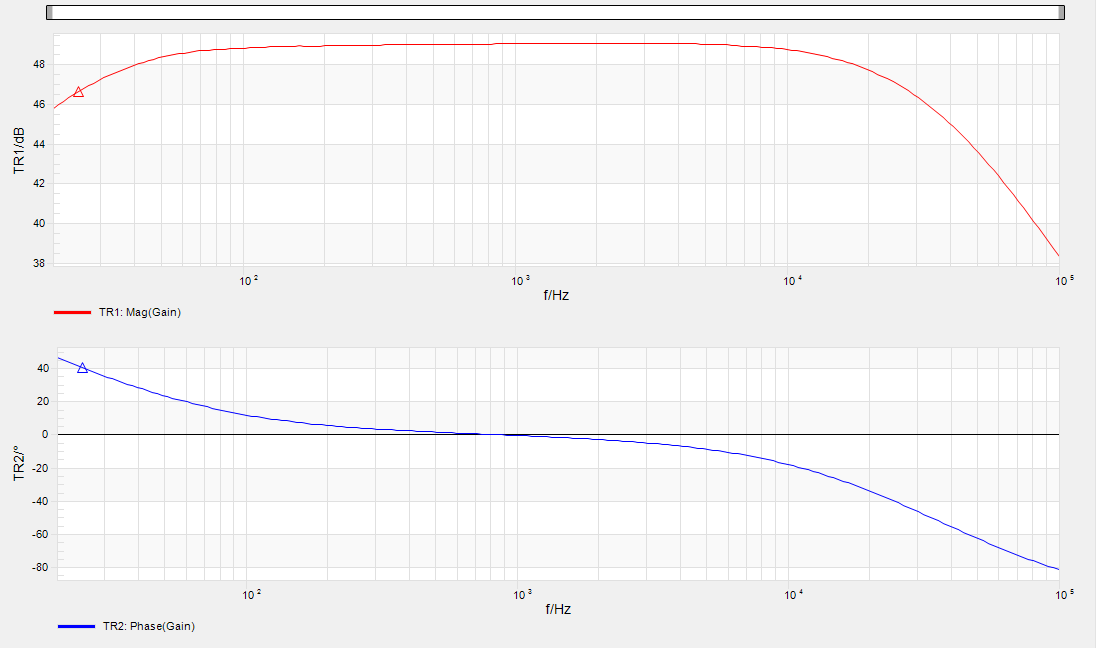
\includegraphics[width=\textwidth]{nkzt10_120324/nkzt10_2.png}
    \caption{Naměřené frekvenční charakteristiky modulu a fáze přenosu}
\end{figure}

\subsection{Měření frekvenční charakteristiky modulu a fáze vstupní impedance (Úkol 3)}

\begin{figure}[H]
    \centering
    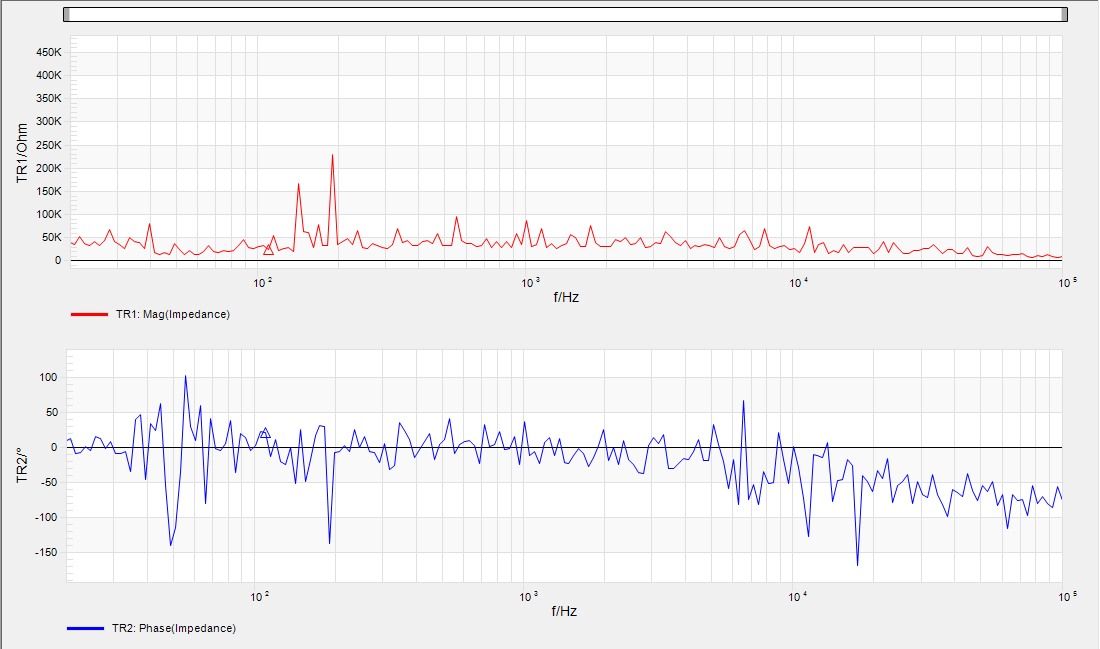
\includegraphics[width=\textwidth]{nkzt10_120324/nkzt10_3.png}
    \caption{Naměřené frekvenční charakteristiky modulu a fáze vstupní impedance}
\end{figure}

\subsection{Měření účinnosti zesilovače (Úkol 4)}

\subsection{Měření harmonického zkreslení na výstupu (Úkol 5)}

\section{Závěr}

\end{document}